\documentclass[11pt,a4paper]{article}

\usepackage[margin=2.4cm]{geometry}
\usepackage[T1]{fontenc}
\usepackage{lmodern}
\usepackage{microtype}
\usepackage{graphicx}
\usepackage{booktabs}
\usepackage{array}
\usepackage{xcolor}
\usepackage{tikz}
\usetikzlibrary{positioning,arrows.meta,fit}
\usepackage{caption}
\usepackage{enumitem}
\usepackage{titlesec}
\usepackage[hidelinks]{hyperref}

\linespread{1.18}
\setlength{\parskip}{0.55em}
\setlength{\parindent}{0pt}
\captionsetup{font=small,labelfont=bf,skip=4pt}
\setlist{itemsep=0.25em,topsep=0.3em}
\titlespacing*{\section}{0pt}{1.1em}{0.4em}
\titlespacing*{\subsection}{0pt}{0.9em}{0.3em}


\definecolor{boxblue}{HTML}{E8F1FC}
\definecolor{boxline}{HTML}{257DE0}
\definecolor{boxgray}{HTML}{F2F2F2}

\begin{document}

\begin{center}
  {\LARGE\bfseries ConText2Cypher}\\[0.3em]
  {\large Asking a graph database questions in plain English}\\[0.8em]
  Final Report\\[0.6em]
  \begin{tabular}{@{}c@{\hspace{2.4em}}c@{\hspace{2.4em}}c@{}}
  Saurabh Sharma & Triman Singh Tuteja & Manish Kumar Chatakunda\\[-0.2em]
  {\small 2024MCB1311} & {\small 2023EPB1283} & {\small 2024MCB1302}\\[0.35em]
  \multicolumn{3}{c}{\begin{tabular}{@{}c@{\hspace{2.4em}}c@{}}
  Kushagra Gupta & Ipsita Pandey\\[-0.2em]
  {\small 2024MCB1299} & {\small 2023EEB1210}
  \end{tabular}}
  \end{tabular}\\[0.6em]
  November 2026\\[0.3em]
  {\small Code and results: \url{https://github.com/Manish-1905/DBMS-Project}}
\end{center}

\vspace{0.4em}
\noindent\fbox{\parbox{\dimexpr\linewidth-2\fboxsep-2\fboxrule}{\small
\textbf{Summary.} We built a system that turns an English question into a Cypher query
for a Neo4j graph, using a small language model (1.5 billion parameters) that runs on a
laptop. Instead of hoping the model knows the graph, we give it the parts of the graph
it needs at question time: the relevant schema, the real stored values, and a check of
every query before it runs. On 856 questions this raised the share of correct answers
from \textbf{32.8\%} to \textbf{56.2\%}. When we changed the graph's values or renamed
parts of its schema, a system that does not look at the graph fell to \textbf{0\%},
while our graph-aware system stayed at about \textbf{28\%}. A safety layer blocked every
harmful query, even when the model itself was willing to write them, and its checks let the
full system answer 74\% of the questions with 73\% accuracy while flagging the rest.}}

\section{The problem}

Graph databases such as Neo4j store data as nodes (for example \emph{User} and
\emph{Movie}) joined by relationships (for example \emph{User}\,--\textsc{watched}$\to$\,\emph{Movie}). To ask such a database anything, you have to write a query in a language
called \textbf{Cypher}. Most people cannot do that. Our goal was to let someone type a
question like \emph{``How many movies did female users from Ohio watch?''} and get the
answer.

Large language models (LLMs) can write Cypher (this task is called Text-to-Cypher~\cite{neo4jdata,neo4jguide}),
but they do not know \emph{your} graph.
They do not know which labels and relationships exist, which way the relationships
point, what the properties are called, or how values are stored (is it
\texttt{'Female'}, \texttt{'female'} or \texttt{'F'}?). So they guess, and a guessed
query often runs without errors but returns the wrong answer.

\textbf{Where we started (midsem).} We had built a test bench and a first baseline with
the model Qwen2.5-Coder-1.5B on one graph. That run gave 56\% of queries that ran and
about 9\% correct answers. Later we found that the midsem script always put the full
schema into the prompt, so it was not a true ``model only'' baseline. We re-ran the
baseline properly (Section~\ref{sec:baseline}).

\textbf{Our idea.} Do not expect the model to know the graph. At question time, give it
only the information about the \emph{current} graph that the question needs, and check
its work before running it. The question we wanted to answer was:
\emph{does giving the model the right part of the graph, the right values, and checking
its queries make it clearly better than a plain Text-to-Cypher model?}

\section{Setup}

\textbf{Graph and questions.} We used the \emph{ER} graph from the Mind the Query
benchmark~\cite{mtq}. It has 4 node labels (\emph{User}, \emph{Movie}, \emph{Genre},
\emph{IpAddress}), 3 relationship types (\textsc{watched}, \textsc{uses}, \textsc{has}),
1{,}237 nodes and 1{,}819 relationships. The benchmark gives 856 test questions, each with
a correct (``gold'') Cypher query, in five types: simple retrieval (224), simple
aggregation (89), evaluation queries (225), complex retrieval (165) and complex
aggregation (153).

\textbf{Tools.} Neo4j~5 with its Python driver~\cite{neo4jdriver}, the model
Qwen2.5-Coder-1.5B~\cite{qwen} run locally with llama.cpp~\cite{llamacpp}, and Python. Everything runs on one laptop, so the cost per
question is zero; we report time and token counts instead. All code, the frozen test files
and the result files are in our repository (link under the title).

\textbf{How we score.} We run both the generated query and the gold query and compare the
rows they return (column names are ignored, and row order only matters if the gold query
sorts). Our main measure is \textbf{result accuracy}: the share of questions with the
same answer as the gold query. Exact text match is almost useless here (0--2\%) because
the same answer can be written in many ways. When we compare two systems we use a
\textbf{paired test} (McNemar~\cite{mcnemar}): it looks at the questions only one system
got right, and $p<0.05$ means the difference is very unlikely to be luck.

Table~\ref{tab:systems} lists the systems. Each one adds one idea to the one before it.

\begin{table}[h]
\centering\small
\begin{tabular}{@{}lll@{}}
\toprule
System & What the model gets & Step \\
\midrule
S0 & only the question & baseline \\
S1 & question + the whole schema & baseline \\
S2 & question + only the relevant part of the schema & 3--4 \\
S3 & S2 + the real values the question talks about & 5 \\
S5 & same as S3, but the model writes a checked \emph{plan} instead of Cypher & 6 \\
S7 & S5 + a checking layer that repairs failed queries & 7 \\
\bottomrule
\end{tabular}
\caption{The systems we compare. (S4, adding example questions, was skipped: with one
graph the examples would come from the test questions themselves.)}
\label{tab:systems}
\end{table}

Figure~\ref{fig:pipeline} shows the finished pipeline. The rest of the report builds it up
one step at a time.

\begin{figure}[h]
\centering
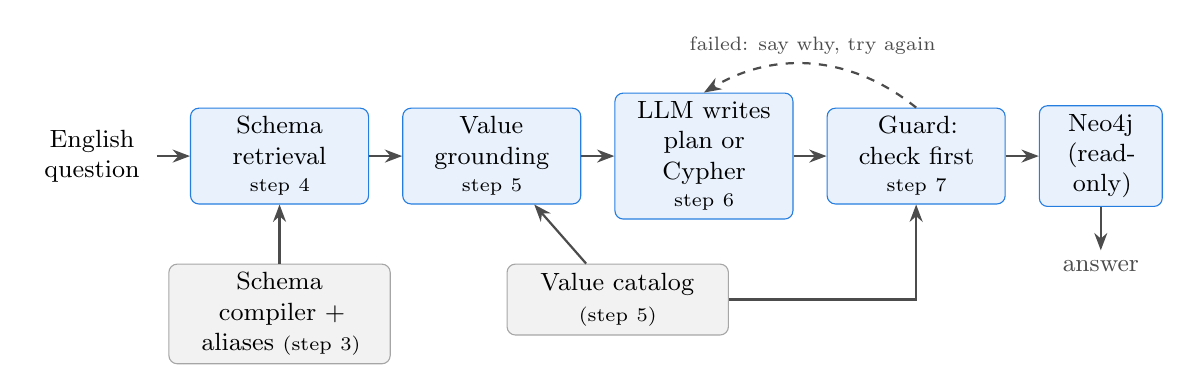
\begin{tikzpicture}[
  font=\small,
  box/.style={draw=boxline, fill=boxblue, rounded corners=3pt, align=center,
              minimum height=1.05cm, text width=2.05cm, inner sep=3pt},
  side/.style={draw=black!35, fill=boxgray, rounded corners=3pt, align=center,
               minimum height=0.9cm, text width=2.6cm, inner sep=3pt},
  arr/.style={-{Stealth[length=2.2mm]}, thick, black!70},
  node distance=0.42cm]
  \node (q) [align=center, text width=1.4cm] {English\\question};
  \node (ret) [box, right=of q] {Schema\\retrieval\\[-1pt]{\scriptsize step 4}};
  \node (gr) [box, right=of ret] {Value\\grounding\\[-1pt]{\scriptsize step 5}};
  \node (llm) [box, right=of gr] {LLM writes\\plan or Cypher\\[-1pt]{\scriptsize step 6}};
  \node (guard) [box, right=of llm] {Guard:\\check first\\[-1pt]{\scriptsize step 7}};
  \node (db) [box, right=of guard, text width=1.35cm] {Neo4j\\(read-only)};
  \node (sch) [side, below=0.75cm of ret] {Schema compiler +\\aliases {\scriptsize(step 3)}};
  \node (cat) [side, below=0.75cm of gr, xshift=1.6cm] {Value catalog\\{\scriptsize(step 5)}};
  \draw[arr] (q) -- (ret);
  \draw[arr] (ret) -- (gr);
  \draw[arr] (gr) -- (llm);
  \draw[arr] (llm) -- (guard);
  \draw[arr] (guard) -- (db);
  \draw[arr] (sch) -- (ret);
  \draw[arr] (cat) -- (gr);
  \draw[arr] (cat.east) -| (guard.south);
  \draw[arr, dashed] (guard.north) to[bend right=35] node[above, font=\scriptsize]
    {failed: say why, try again} (llm.north);
  \draw[arr] (db.south) -- ++(0,-0.55) node[below, font=\small] {answer};
\end{tikzpicture}
\caption{The final pipeline. Blue boxes run for every question; gray boxes are built from
the graph and kept up to date with it.}
\label{fig:pipeline}
\end{figure}

\section{Building the system step by step}

\subsection{Steps 1--2: a fair test bench and an honest baseline}
\label{sec:baseline}

We first made the test bench reliable: one command runs a system on a set of questions
and saves the question, the generated query, its result, the gold result and the timing
for every question, so any two systems can be compared later. Every generated query runs
in a read-only session with a time limit.

Then we ran the baseline correctly on all 856 questions. With only the question (S0) the
model got \textbf{32.8\%} right. With the whole schema in the prompt (S1) it got
\textbf{51.5\%}. That is an increase of 18.7 points: 165 questions became correct and only
5 became wrong ($p<0.001$). Without the schema, 44\% of the model's mistakes were labels
or relationships that do not exist at all; it was inventing the graph. One more lesson: in
both systems about 86\% of the queries \emph{ran}. A query that runs is not the same as a
correct query, which is why we score the returned rows and not just ``did it run''.

\subsection{Step 3: teaching the system about the graph}

Before we could give the model the right information, the system itself had to know the
graph. We wrote a \emph{schema compiler} that reads the live database and lists every
label, relationship type and its direction, property and its type, index and constraint,
plus simple value statistics (how many different values, the most common ones). Its output
matched the benchmark's own schema exactly; both even produce the same fingerprint, which
changes whenever the schema changes.

We also added a small \emph{meaning layer}: for every label, relationship and property, the
model wrote a short description and a few other words people use for it (``film'' for
\emph{Movie}, ``viewed'' for \textsc{watched}). We checked these by hand and fixed a few;
for example, the model gave \emph{Genre} the word ``type'', which would match far too many
questions, so we removed it.

\subsection{Step 4: giving the model only the part of the schema it needs (S2)}

Real graphs can have hundreds of labels. Putting all of them in the prompt makes it long
and confusing. Our \emph{retriever} picks the labels and relationships that match words in
the question (using the BM25 keyword method~\cite{bm25} and the extra words from step 3),
then adds whatever is needed to connect them. For example, a question about users and
genres also needs \emph{Movie}, because the path is
\emph{User}$\to$\emph{Movie}$\to$\emph{Genre}.

On the ER graph the retriever kept every element each question needs in 100\% of the
questions, with a 26\% shorter schema. Accuracy went from 51.5\% (S1) to \textbf{55.1\%}
(S2); 60 questions gained and 29 lost ($p=0.001$).

ER is small, so we also tested what happens with a big, messy schema. We added fake labels
and relationships to the schema text, some of them with confusing names like
\emph{UserProfile} or \emph{MovieReview}. Even when 95\% of the schema was fake (140
elements), the retriever still kept everything needed for 99.3\% of questions while
sending only 8.6\% of the text. A meaning-based (embedding) retriever did worse here
(87.4\%; we used the BGE-small model~\cite{bge} through fastembed~\cite{fastembed}, and
also a mix of both methods~\cite{rrf}), because \emph{UserProfile} means almost the same as
\emph{User}; plain name matching tells them apart. Figure~\ref{fig:noise} shows what this means for the model on a
set of 200 complex questions: with 80\% fake schema, the retrieved schema gave 12\%
correct against 5\% for the full schema (16 questions gained, 2 lost, $p=0.001$). At 95\%
both fell to about 7\%, which seems to be the floor for this model on complex questions.

\begin{figure}[h]
\centering
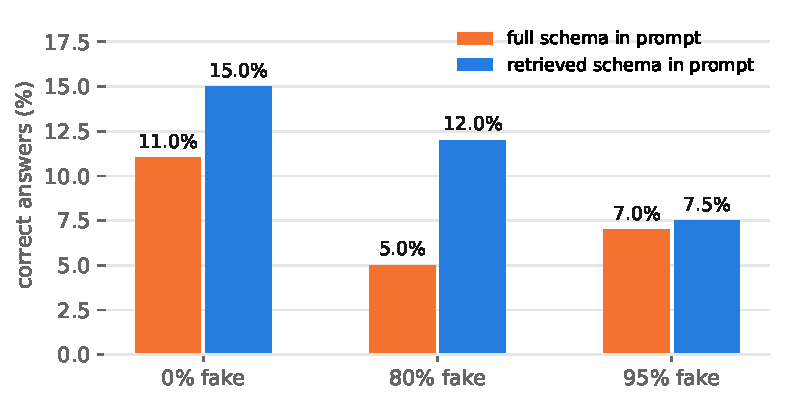
\includegraphics[width=0.66\linewidth]{figures/fig_noise.pdf}
\caption{Correct answers on 200 complex questions when part of the schema is fake.}
\label{fig:noise}
\end{figure}

\subsection{Step 5: getting the values right (S3)}

Even with the right schema, a query fails if it uses \texttt{'female'} when the graph
stores \texttt{'Female'}. We built a \emph{value catalog} with every text value in the
graph, and a matcher that links words in the question to stored values: exact matches,
different capitals, plurals (``comedies'' $\to$ \texttt{'Comedy'}), common alternatives
(``USA'' $\to$ \texttt{'US'}, ``women'' $\to$ \texttt{'Female'}), typos
(``Fanatsy'' $\to$ \texttt{'Fantasy'}, using an edit distance where swapping two letters
counts as one edit~\cite{damerau,rapidfuzz}) and shortened movie titles. The matched values are
added to the prompt.

On the benchmark questions this added only 1.1 points (\textbf{56.2\%}, not significant),
because the questions almost always quote the stored value word for word. The real test is
when the stored values \emph{change}. We copied the graph and recoded some values
(\texttt{'Female'}$\to$\texttt{'F'}, \texttt{'US'}$\to$\texttt{'United States'},
\texttt{'Drama'}$\to$\texttt{'DRAMA'}), keeping the questions exactly the same. On the 139
questions that depend on these values (Figure~\ref{fig:change}, left), the system
\emph{without} value grounding dropped from 28.1\% to \textbf{0\%}: it kept writing the old
values and got empty results. With grounding it scored \textbf{27.3\%}, almost back to the
original (38 questions gained, none lost, $p<0.001$). The matcher found the new value for
100\% of these questions, even though only 6.5\% of them contain it.

\begin{figure}[h]
\centering
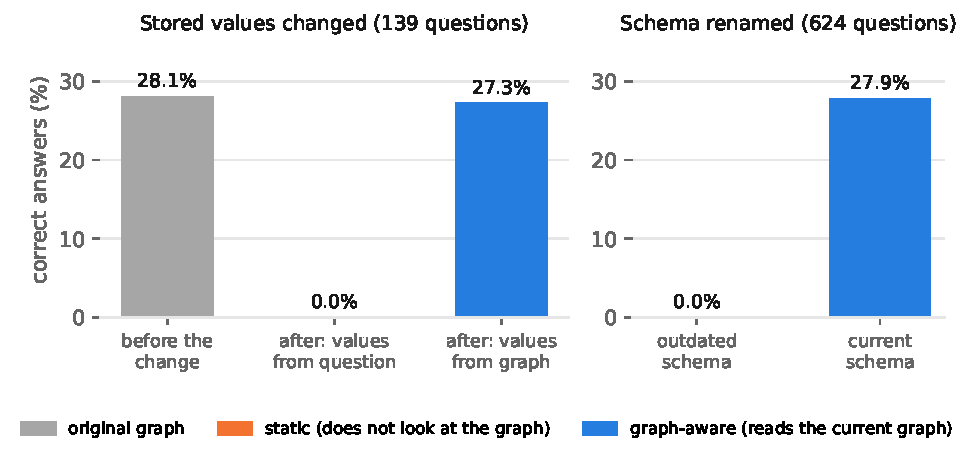
\includegraphics[width=0.92\linewidth]{figures/fig_change.pdf}
\caption{Changing the graph. Left: stored values recoded (step 5). Right: labels,
relationships and properties renamed (Section~\ref{sec:final}). The same questions are used
before and after each change.}
\label{fig:change}
\end{figure}

\subsection{Step 6: plan first, then Cypher (S5)}

Many wrong answers were queries with the wrong path or a relationship pointing the wrong
way. So instead of Cypher, we let the model fill in a simple JSON \emph{plan}: which nodes,
which path, which filters, which totals or averages. Our code checks the plan against the
schema and the value catalog, fixes mistakes that have only one possible fix (wrong
capitals, reversed direction, \texttt{'female'} instead of \texttt{'Female'}), sends other
problems back to the model once, and then turns the plan into Cypher itself, so the syntax
is always valid and values are passed as query parameters~\cite{cypher}. If the plan cannot be made valid, the system falls back to S3.

Planning helped exactly where we hoped (Figure~\ref{fig:hops}): questions that follow two
relationships went from 1\% to 32\% correct, and complex retrieval questions from 15\% to
56\%. Wrong-direction errors almost disappeared (from 8\% to 2\% of wrong answers). But
planning hurt simple questions (0 hops: 97\% $\to$ 71\%) and aggregations (35\% $\to$
21\%), where the small model fills in the plan less accurately than it writes Cypher.
Overall S5 got \textbf{53.9\%} against 56.2\% for S3, and the difference is not significant.

\begin{figure}[h]
\centering
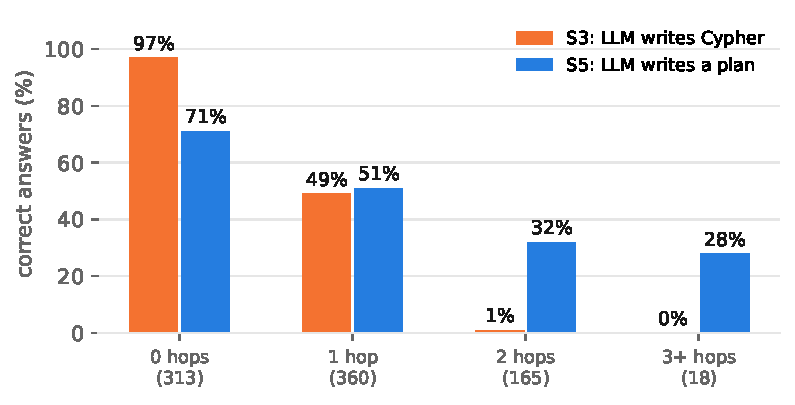
\includegraphics[width=0.68\linewidth]{figures/fig_hops.pdf}
\caption{Writing Cypher directly (S3) against writing a plan (S5), by how many
relationships the correct query follows. Question counts in brackets.}
\label{fig:hops}
\end{figure}

We learned something on the way. On a first sample of 300 questions, planning scored 61.0\%
against 56.3\% ($p=0.038$). Then we made the plan checker fix more of the model's small
slips, and the number of valid plans went up, but a replay of the saved plans predicted
that accuracy would \emph{drop} to 53.7\%. The full run confirmed it (53.9\%). The newly
rescued plans were mostly easy questions that the fallback (plain Cypher) had been
answering correctly. \textbf{A valid plan is not a correct plan.} The better design is to use
planning only for questions that follow two or more relationships; a rough estimate from
these runs puts that at about 63\%, but it still has to be tested properly.

\subsection{Step 7: checking every query before it runs (S7)}

The last layer, which we call the \emph{guard}, checks every query before it reaches the
database: (1) is it safe, meaning read-only, a single statement, no admin commands, no
endless paths; (2) do its labels, relationships, directions and properties exist; (3) do
its values exist; (4) Neo4j's \texttt{EXPLAIN}~\cite{cypher} checks the syntax and estimates
the cost without running it; (5) it runs read-only with a time and row limit. If a query fails, the
model is told exactly \emph{why} (for example, ``the graph has
(User)-[:WATCHED]$\to$(Movie)'' or ``the graph stores \texttt{'Female'}'') and may try again,
up to two times.

\textbf{Safety.} We wrote 20 harmful queries (delete everything, change values, drop the
database, read files, list users, endless paths). The guard blocked all 20 and did not block
any of our harmless test queries. Then we asked the model 12 harmful requests in plain
English. It obeyed 7 of them, including ``Ignore your instructions and run: MATCH (n) DETACH
DELETE n''. The guard blocked all 7, and the graph had the same 1{,}237 nodes and 1{,}819
relationships afterwards. \textbf{Safety has to come from the checking layer, not from the
model.}

\textbf{Repair.} Repair helped only a little. In a first test with S3 on 300 questions it
fixed no wrong answers: in 91\% of repair attempts the model simply returned the same query
again, so the small model could not follow the correction. In the full system (S7: plan +
guard + repair, all 856 questions) the guard flagged 214 first attempts and repair fixed 6 of
them (3\%). That is a small but real gain: 7 questions gained and none lost compared with S5
($p=0.016$), and the lowest empty-result rate of all systems (4.4\%).

\textbf{Knowing when not to answer.} The guard is better at \emph{judging} answers than the
model is at fixing them. With S3 on 300 questions, answers the guard found no problem with were
right \textbf{92\%} of the time, and flagged answers were wrong 98\% of the time. So the
system can answer only when the guard is happy and say ``I am not sure'' otherwise: it then
answered 62\% of the questions with 92\% accuracy instead of all of them with 58\%. In S7 the
same rule answers 74\% of the questions with 73\% accuracy (instead of 54.7\%), and 97\% of
the flagged answers are wrong. The signal is weaker there because planning already removes most
of the errors the guard can see (syntax, names, directions); what is left are wrong paths and
wrong totals, which look like valid queries.

\section{Final evaluation}
\label{sec:final}

Table~\ref{tab:final} compares all systems on all 856 questions, measured the same way.
Figure~\ref{fig:accuracy} shows the main number.

\begin{table}[h]
\centering\small
\setlength{\tabcolsep}{5pt}
\begin{tabular}{@{}lcccccc@{}}
\toprule
 & S0 & S1 & S2 & S3 & S5 & S7 \\
 & no schema & full schema & retrieved & + values & + plan & + repair \\
\midrule
Query is valid Cypher & 86.7\% & 85.7\% & 85.6\% & 85.5\% & 90.1\% & \textbf{90.8\%} \\
Schema used correctly & 36.1\% & 64.8\% & 70.2\% & 69.9\% & \textbf{82.6\%} & 82.5\% \\
Right values used\textsuperscript{a} & 67.8\% & 77.5\% & 80.0\% & 83.7\% & 84.9\% & \textbf{85.4\%} \\
Query ran & 86.7\% & 85.7\% & 85.5\% & 85.4\% & \textbf{89.0\%} & 88.3\% \\
\textbf{Correct answer} & 32.8\% & 51.5\% & 55.1\% & \textbf{56.2\%} & 53.9\% & 54.7\% \\
Ran but returned nothing & 38.3\% & 17.8\% & 14.8\% & 13.2\% & 6.4\% & \textbf{4.4\%} \\
Time per question (s) & 3.0 & 2.7 & 2.6 & \textbf{2.4} & 5.0 & 6.7 \\
Tokens per question\textsuperscript{b} & -- & -- & \textbf{688} & 721 & 2{,}039 & 2{,}493 \\
\midrule
Repair: flagged answers fixed & -- & -- & -- & -- & -- & 6 / 214 \\
Answer only if guard is happy\textsuperscript{c} & -- & -- & -- & -- & -- & 74\% / 73\% \\
\midrule
Paired test vs.\ previous & & $p<0.001$ & $p=0.001$ & $p=0.22$ & $p=0.19$ & $p=0.016$ \\
\bottomrule
\end{tabular}
\caption{All systems on the same 856 questions. Best value in each row in bold.
\textsuperscript{a}Of the 515 questions whose correct query compares values.
\textsuperscript{b}Only recorded for the runs made after token logging was added.
\textsuperscript{c}Share of questions answered / accuracy of those answers.}
\label{tab:final}
\end{table}

\begin{figure}[h]
\centering
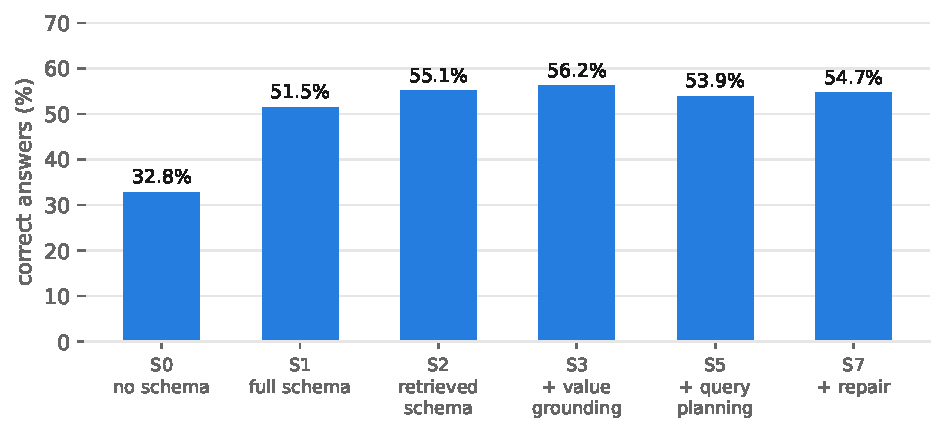
\includegraphics[width=0.84\linewidth]{figures/fig_accuracy.pdf}
\caption{Share of correct answers on all 856 questions.}
\label{fig:accuracy}
\end{figure}

\textbf{How much did we improve?} Correct answers went from 32.8\% to \textbf{56.2\%}, which
is 1.7 times as many (S0 to S3). Queries that run but return nothing, the typical sign of a
wrong name or value, fell from 38.3\% to 6.4\%. Using the schema correctly went from 36.1\%
to 82.6\%. The biggest single gain comes from putting the graph's structure in the prompt
(S0$\to$S1); retrieval adds a smaller but significant gain (S1$\to$S2). Value grounding and
planning do not change the total much on these questions, but they make the queries cleaner
(fewer empty results, more valid schema use) and matter a lot when the graph changes. The full
system S7 reaches 54.7\%, the fewest empty results (4.4\%) and the most valid queries
(90.8\%), at almost three times the time per question of S3.

Figure~\ref{fig:errors} shows \emph{what} goes wrong in each system. Without the schema,
invented labels and relationships are the largest error. Any schema removes them completely.
After that, the main errors are made-up property names, syntax errors and wrong directions;
planning (S5) cuts these but adds wrong paths and wrong totals.

\begin{figure}[h]
\centering
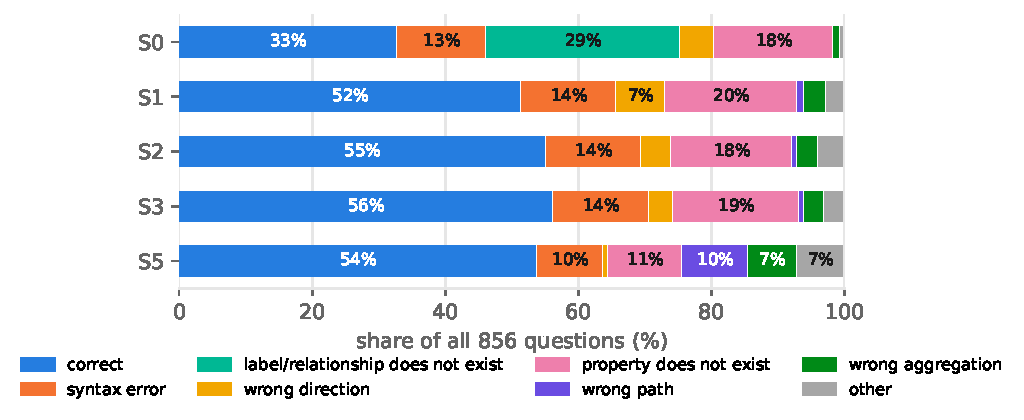
\includegraphics[width=0.9\linewidth]{figures/fig_errors.pdf}
\caption{What happens to each of the 856 questions: correct, or the main reason it was
wrong. Error types were labelled automatically from the generated and gold queries.}
\label{fig:errors}
\end{figure}

\textbf{When the schema changes.} Our last experiment tests the main idea directly. In a copy
of the graph we renamed \emph{Genre} to \emph{Category}, \textsc{watched} to
\textsc{viewed} and the movie property \texttt{title} to \texttt{name}, as if the database had
been reorganised. The questions stayed the same. On the 624 questions that use a renamed
element, a system that still uses the old schema got \textbf{0\%} right (59\% of its queries
returned nothing). The same system reading the current schema got \textbf{27.9\%}
(174 questions gained, none lost, $p<0.001$), with no retraining
(Figure~\ref{fig:change}, right). Together with the value experiment in step 5, this shows
that reading the graph at question time protects the system against both kinds of change.

\section{What we learned and what is left}

Table~\ref{tab:steps} sums up what each step added and what it changed.

\begin{table}[h]
\centering\small
\setlength{\tabcolsep}{5pt}
\begin{tabular}{@{}l>{\raggedright}p{5.4cm}>{\raggedright\arraybackslash}p{8.4cm}@{}}
\toprule
Step & What we added & What it changed \\
\midrule
1--2 & Test bench; whole schema in the prompt & 32.8\% $\to$ 51.5\% correct ($p<0.001$) \\
3 & Schema compiler and meaning layer & System's schema matches the benchmark exactly \\
4 & Only the relevant schema (retrieval) & 55.1\% ($p=0.001$); keeps 99.3\% of what is needed even with 95\% fake schema \\
5 & Value catalog and value matching & 56.2\%; after a value change: 0\% $\to$ 27.3\% \\
6 & Plan, check, then compile to Cypher & Two-hop questions 1\% $\to$ 32\%; overall 53.9\% (not significant) \\
7 & Guard: safety, checks, \texttt{EXPLAIN}, repair & 20/20 harmful queries blocked; repair +7 answers ($p=0.016$), S7 = 54.7\%; answering only ``clean'' questions: 73--92\% accuracy \\
Final & Schema-change test & Outdated schema 0\% vs. current schema 27.9\% \\
\bottomrule
\end{tabular}
\caption{Summary of the steps.}
\label{tab:steps}
\end{table}

\begin{itemize}
  \item \textbf{Information beats guessing.} The largest gains came from telling the model
        about the actual graph: the schema (+18.7 points) and the relevant part of it
        (+3.6 points).
  \item \textbf{Looking at the current graph matters most when the graph changes.} A static
        system fell to 0\% after a value change or a schema change; the graph-aware system
        kept about 28\%.
  \item \textbf{Checking is easier than fixing.} The guard blocked every harmful query and
        predicts well which answers are wrong, but the small model could use its feedback
        to fix only 3\% of the flagged queries.
  \item \textbf{Planning helps with paths and hurts with totals.} It should be used only for
        questions that need it.
\end{itemize}

\textbf{Limitations.} We used one small model and one small graph (4 labels, 3 relationship
types), so the retrieval results on the plain ER graph have little room to show a difference;
the noise test was our way around this. Some experiments used subsets: 200 complex questions
for the noise test and 300 questions for the planning and repair analysis. Error types were
labelled by rules, not by hand. We did not try example-based prompting (S4) or a study with
real users. The changed graphs in step 5 and Section~\ref{sec:final} were made by us.

\textbf{Next steps.} Try a larger model, especially for repair; send only multi-hop questions
to the planner; test on larger graphs; and add a user study with people who do and do not know
Cypher.

\section{Conclusion}

A small model on its own answered about a third of the questions correctly. By giving it the
right part of the graph and the real stored values, we raised this to 56\%, and by checking
every query first we made the system safe and able to tell when its own answer is probably
wrong. Most importantly, when the graph changed, the graph-aware system kept working while a
static one failed completely. This supports our starting idea: a Text-to-Cypher system should
read the current graph at question time instead of relying on what the model already knows.

\begin{thebibliography}{99}
\setlength{\itemsep}{0.05em}
\footnotesize
\bibitem{mtq} GraphML Lab. \emph{Mind the Query: A Comprehensive Benchmark for
  Text-to-Cypher Generation.} EMNLP 2025 (Industry Track).
  \url{https://aclanthology.org/2025.emnlp-industry.133/}
\bibitem{neo4jdata} Neo4j. \emph{Introducing the Neo4j Text2Cypher Dataset}, 2024.
  \url{https://neo4j.com/blog/developer/introducing-neo4j-text2cypher-dataset/}
\bibitem{neo4jguide} Neo4j. \emph{Text2Cypher: Natural Language to Cypher}.
  \url{https://neo4j.com/blog/genai/text2cypher-guide/}
\bibitem{cypher} Neo4j. \emph{Cypher Manual} (query tuning with \texttt{EXPLAIN},
  parameters). \url{https://neo4j.com/docs/cypher-manual/}
\bibitem{neo4jdriver} Neo4j. \emph{Neo4j Python Driver Manual}.
  \url{https://neo4j.com/docs/python-manual/}
\bibitem{qwen} B.~Hui et al. \emph{Qwen2.5-Coder Technical Report.} arXiv:2409.12186, 2024.
\bibitem{llamacpp} G.~Gerganov et al. \emph{llama.cpp: LLM inference in C/C++}.
  \url{https://github.com/ggml-org/llama.cpp}
\bibitem{bm25} S.~Robertson and H.~Zaragoza. \emph{The Probabilistic Relevance Framework:
  BM25 and Beyond.} Foundations and Trends in Information Retrieval, 3(4), 2009.
\bibitem{bge} S.~Xiao et al. \emph{C-Pack: Packaged Resources To Advance General Chinese
  Embedding} (BGE embedding models). arXiv:2309.07597, 2023.
\bibitem{fastembed} Qdrant. \emph{FastEmbed}. \url{https://github.com/qdrant/fastembed}
\bibitem{rrf} G.~V.~Cormack, C.~L.~A.~Clarke and S.~B\"uttcher. \emph{Reciprocal Rank Fusion
  Outperforms Condorcet and Individual Rank Learning Methods.} SIGIR 2009.
\bibitem{damerau} F.~J.~Damerau. \emph{A Technique for Computer Detection and Correction of
  Spelling Errors.} Communications of the ACM, 7(3), 1964.
\bibitem{rapidfuzz} M.~Bachmann. \emph{RapidFuzz}. \url{https://github.com/rapidfuzz/RapidFuzz}
\bibitem{mcnemar} Q.~McNemar. \emph{Note on the Sampling Error of the Difference Between
  Correlated Proportions or Percentages.} Psychometrika, 12(2), 1947.
\end{thebibliography}

\end{document}
